%% Examples of SingularityNET AI Service Assemblages
%%
%% Render with:
%% pdflatex -shell-escape snet-service-assemblages.tex

\documentclass[]{article}
\usepackage{url}
\usepackage{minted}
\usepackage[hyperindex,breaklinks]{hyperref}
\usepackage{breakurl}
\usepackage{listings}
\lstset{basicstyle=\ttfamily\footnotesize,breaklines=false,frame=single}
\usepackage{float}
\restylefloat{table}
\usepackage{longtable}
\usepackage{graphicx}
\usepackage[font=small,labelfont=bf]{caption}
\usepackage[skip=0pt]{subcaption}
\usepackage{circledsteps}

\begin{document}

\title{Examples of SingularityNET AI Service Assemblages}
\author{Nil Geisweiller}
\maketitle

\section{Introduction}
This document goes over a list of potential AI service assemblages
that could be used as test cases for the next phase.  Nearly all AI
services involved already exist on the SingularityNET platform.

\section{AI Services Assemblages}
Each assemblage is shown with:
\begin{enumerate}
\item a flowchart, arrows representing the flow of information between
  AI services represented as blue boxes;
\item a type signature using types provided by an imaginary possible
  future version of the AI-DSL, for now expressed in Idris;
\item optionally an implementation of such assemblage, again expressed
  in Idris.
\end{enumerate}

\subsection{Recognize Emotion of Hand Written Text}
Let's begin with an assemblage of two services to recognize the
emotion of hand written text.  Given an image of handwritten text, it
first turns it into a string of text, then recognize an emotion from
that.
\begin{figure}[H]
  \centering
  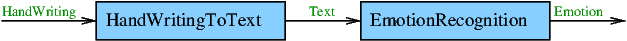
\includegraphics[scale=0.55]{figs/HandWritingEmotionRecognition.png}
\end{figure}
\begin{minted}[mathescape]{idris}
handwritingEmotionRecognition : HandWriting -> Emotion
handwritingEmotionRecognition = emotionRecognition . handWritingToText
\end{minted}
The type \texttt{HandWriting} could be specialized type of image and
\texttt{Emotion} could be a category, or possibly categorical
distribution, of emotions.  The composition operator \texttt{.} can be
used for the implementation given the simplicity of the assemblage.

\subsection{Topic Analysis of Speech}
\begin{figure}[H]
  \centering
  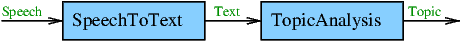
\includegraphics[scale=0.55]{figs/SpeechTopicAnalysis.png}
\end{figure}
\begin{minted}[mathescape]{idris}
speechTopicAnalysis : Speech -> Topic
speechTopicAnalysis = topicAnalysis . speechToText
\end{minted}
\texttt{Speech} could be a special type of sound and \texttt{Topic} a
special type of text, or maybe category, or categorical distribution,
of topics.

\subsection{Topic Analysis of Text from Any Language}
This assemblage is simply doing topic analysis but for any language by
translating the input text into English and the output topic back into
the original language.
\begin{figure}[H]
  \centering
  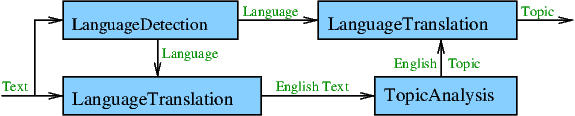
\includegraphics[scale=0.55]{figs/AnyLanguageTopicAnalysis.png}
\end{figure}
\begin{minted}[mathescape]{idris}
anyLanguageTopicAnalyzer : Text -> (l : Language ** Topic l)
anyLanguageTopicAnalyzer = ?h
anyLanguageTopicAnalyzer' : Text l -> Topic l
anyLanguageTopicAnalyzer' = ?h
\end{minted}
We offer two definitions:
\begin{enumerate}
\item \texttt{anyLanguageTopicAnalyzer}: corresponding exactly to its
  flowchart;
\item \texttt{anyLanguageTopicAnalyzer'}: corresponding to that
  flowchart without language detection.
\end{enumerate}
There is an interesting use of dependent types here.  In the first
definition, \texttt{anyLanguageTopicAnalyzer}, a dependent pair is
used to return the recognized language then passed to \texttt{Topic},
here a parameterized type, to specify its language.  In the second
definition, \texttt{anyLanguageTopicAnalyzer'}, a type variable is
used to express the guaranty that the language of the output topic is
the same as the one of the text.

\subsection{Recognize Emotion from Speech}
That assemblage combines a Speech Emotion Recognition service with a
sub-assemblage of speech-to-text and text-emotion-recognition
services.  The idea is that such assemblage would improve the
performance of emotion recognition by combining different services and
aggregating their results.
\begin{figure}[H]
  \centering
  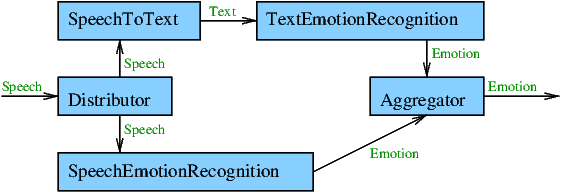
\includegraphics[scale=0.55]{figs/SpeechEmotionRecognition.png}
\end{figure}
\begin{minted}[mathescape]{idris}
speechEmotionRecognizer : Speech -> Emotion
speechEmotionRecognizer = ?h
\end{minted}

\subsection{Turn an English Song into a Chinese Song}
This assemblage aims at turning an English song into the same song but
sang in Chinese.
\begin{figure}[H]
  \centering
  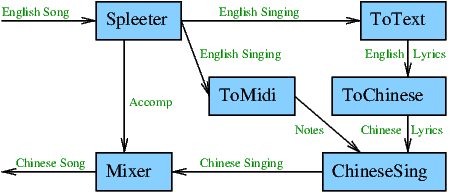
\includegraphics[scale=0.55]{figs/EnglishToChineseSong.png}
\end{figure}
\begin{minted}[mathescape]{idris}
englishSongToChineseSong : Song English -> Song Chinese
englishSongToChineseSong x = let (enSing, accomp) = Spleeter x
                                 enLyrics = toText enSing
                                 chLyrics = toChinese enLyrics
                                 notes = toMidi enSing
                                 chSing = chineseSing notes chLyrics
                             in accomp + chSing
Spleeter : Song l -> (Singing l, Intrumental)
Spleeter song = ?h
\end{minted}
Note the use of the parameterized type \texttt{Song} that could be a
specialized type of audio, a song in a given language.  The
implementation involves the \texttt{let} construct.  There are
certainly ways to replace that by something purely compositional,
something we may want to consider to make the AI-DSL language more
composition friendly.  In addition we provide an example of type
signature of the AI service \texttt{Spleeter}, using dependent types
again.

All services involved in that assemblage with the exception of
\texttt{toMidi} exist on SingularityNET.  To create \texttt{toMidi} we
have however found a number of open source projects that could
potentially be used
\begin{itemize}
\item
  \href{https://basicpitch.spotify.com}{https://basicpitch.spotify.com}
  (Apache license);
\item
  \href{https://github.com/NFJones/audio-to-midi}{https://github.com/NFJones/audio-to-midi}
  (MIT license);
\item
  \href{https://github.com/NFJones/audio-to-midi}{https://aubio.org/}
  (GPL license);
\item
  \href{https://wave2mid.sourceforge.net/index-en.html}{https://wave2mid.sourceforge.net/index-en.html}
  (unknown license);
\item
  \href{https://github.com/justinsalamon/audio\_to\_midi\_melodia}{https://github.com/justinsalamon/audio\_to\_midi\_melodia}
  (unknown license);
\item
  \href{https://github.com/bill317996/Audio-to-midi}{https://github.com/bill317996/Audio-to-midi}
  (MIT license);
\item
  \href{https://github.com/emredjan/audio-to-midi}{https://github.com/emredjan/audio-to-midi}
  (unknown license)
\item
  \href{https://github.com/sbaeunker/audioToMidiConverter}{https://github.com/sbaeunker/audioToMidiConverter}
  (GPL license)
\end{itemize}

\section{conclusion}
The type signatures are fairly simple in these examples, they could of
course be made more sophisticated, or additional properties could be
added.  These aspects are important and have been previously explored
to some degree.  But they will likely not be the main focus of the
next phase, so are left out or simplified for now.  The purpose of the
next phase will be to build a rudimentary, yet working from
end-to-end, AI-DSL prototype.
\end{document}
